\section{Evaluation}
This preview section now reflects the corrected targeted measurements generated under hardware SGX for both MNT224 and A1. The table inputs are synchronized with the targeted-table pipeline so we can inspect the paper-style layout with the updated data.

\subsection{Theory Comparison}
\begin{table*}[t]
\centering
\caption{Theory comparison of representative revocable policy-based chameleon hash schemes.}
\scriptsize
\TableStyle
\resizebox{\textwidth}{!}{\begin{tabular}{lccc}
\toprule
\textbf{Scheme} & \textbf{KeyGen} & \textbf{Hash} & \textbf{Adapt / Revocation Path} \\
\midrule
FB-PCH & $O(|S|)$ & $O(|policy|)$ & $O(|policy|)$ \\
EHR-RPCH & $O(|S|+\log N)$ & $O(|policy|)$ & KGC token + server ciphertext update \\
PNITCH & $O(|S|)$ & $O(|policy|)$ & authorization token + adapt \\
RPCH-XNM'21 & $O(|S|+\log N)$ & $O(|policy|)$ & $O(|policy|+\log N)$ \\
TAR-PCH & $O(|S|+\log N)$ & $O(|policy|)$ & KGC trace + server update \\
TPCH & $O(|S|+\log N)$ & $O(|policy|)$ & $O(|policy|+\log N)$ \\
TEE-RPCH & $O(|S|)$ & $O(|policy|)$ & server Transform1 + TEE Transform2/check + user hash-check \\
\bottomrule
\end{tabular}
}
\end{table*}

\subsection{Baseline Comparison}
We compare the corrected split design $\textsf{CHET-2OA}+\textsf{ABE-2OD}$ with the no-cloud baseline $\textsf{CHET-OA}+\textsf{ABE-OD}$. The server, TEE, and modifier columns are reported separately to match the actual implementation split.

\begin{figure*}[t]
\centering
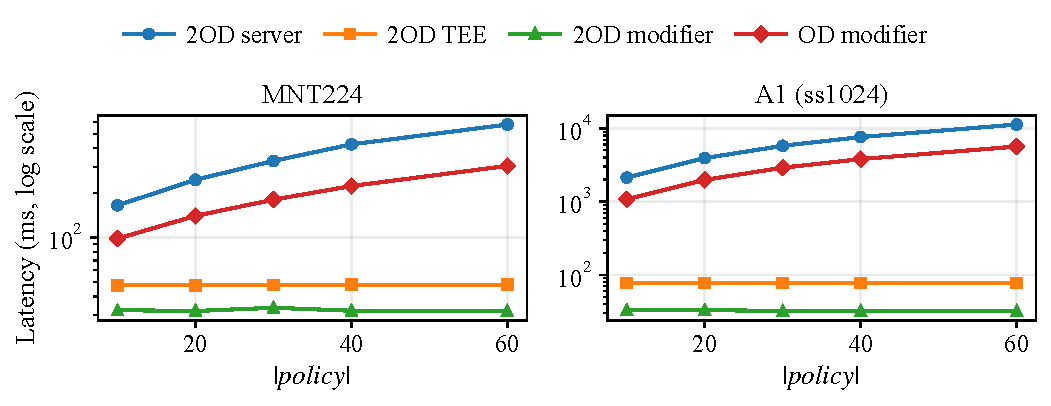
\includegraphics[width=0.84\textwidth]{../targeted_tables/figures/adaptation_latency.pdf}
\caption{Adaptation latency split on MNT224 and A1.}
\label{fig:targeted-adaptation}
\end{figure*}

\begin{table*}[t]
\centering
\caption{Adaptation latency across policy sizes (ms), $|\mathbb{S}|=60$.}
\scriptsize
\TableStyle
\resizebox{\textwidth}{!}{\begin{tabular}{c rr rr rr rr rr}
\toprule
\multirow{3}{*}{$|policy|$} & \multicolumn{6}{c}{\textbf{CHET-2OA + ABE-2OD}} & \multicolumn{4}{c}{\textbf{CHET-OA + ABE-OD}} \\
\cmidrule(lr){2-7}\cmidrule(lr){8-11}
 & \multicolumn{2}{c}{\textbf{Server}} & \multicolumn{2}{c}{\textbf{TEE}} & \multicolumn{2}{c}{\textbf{Modifier}} & \multicolumn{2}{c}{\textbf{TEE}} & \multicolumn{2}{c}{\textbf{Modifier}} \\
\cmidrule(lr){2-3}\cmidrule(lr){4-5}\cmidrule(lr){6-7}\cmidrule(lr){8-9}\cmidrule(lr){10-11}
 & \textbf{MNT} & \textbf{A1} & \textbf{MNT} & \textbf{A1} & \textbf{MNT} & \textbf{A1} & \textbf{MNT} & \textbf{A1} & \textbf{MNT} & \textbf{A1} \\
\midrule
10 & 164.9 & 2127.3 & 47.6 & 77.5 & 32.3 & 33.0 & 50.7 & 79.6 & 98.3 & 1071.1 \\
20 & 245.3 & 3915.3 & 47.6 & 77.5 & 31.9 & 33.0 & 51.8 & 80.6 & 140.0 & 1976.3 \\
30 & 329.2 & 5766.7 & 47.7 & 77.4 & 33.6 & 32.2 & 50.4 & 79.6 & 180.2 & 2899.0 \\
40 & 425.5 & 7588.3 & 48.0 & 77.2 & 32.0 & 32.3 & 50.6 & 80.2 & 222.6 & 3797.3 \\
60 & 579.1 & 11248.6 & 47.9 & 77.5 & 31.9 & 32.1 & 50.1 & 79.3 & 304.7 & 5636.2 \\
\bottomrule
\end{tabular}
}
\label{tab:targeted-adaptation}
\end{table*}

\subsection{Hash-check Benefit}
We also isolate the user-side benefit of the final hash-check trick. The strict legacy comparison now measures a full re-encryption-based finalize path rather than the earlier lightweight AES-only check.

\begin{figure*}[t]
\centering
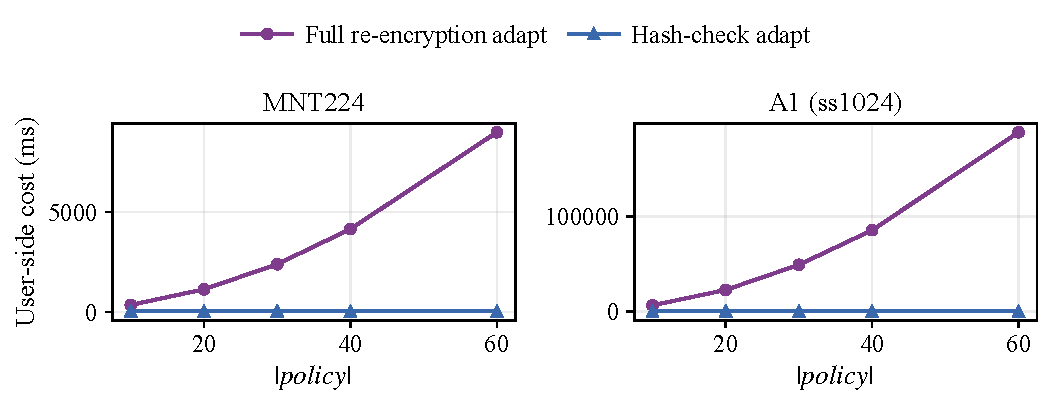
\includegraphics[width=0.84\textwidth]{../targeted_tables/figures/hashcheck_vs_reenc.pdf}
\caption{Full re-encryption finalization versus hash-check finalization.}
\label{fig:targeted-hashcheck}
\end{figure*}

\begin{table*}[t]
\centering
\caption{User-side finalization comparison (ms).}
\scriptsize
\TableStyle
\resizebox{\textwidth}{!}{\begin{tabular}{c rr rr}
\toprule
\multirow{2}{*}{$|policy|$} & \multicolumn{2}{c}{\textbf{Full Re-encryption Adapt}} & \multicolumn{2}{c}{\textbf{Hash-check Adapt}} \\
\cmidrule(lr){2-3}\cmidrule(lr){4-5}
 & \textbf{MNT} & \textbf{A1} & \textbf{MNT} & \textbf{A1} \\
\midrule
10 & 355.1 & 6427.3 & 32.3 & 33.0 \\
20 & 1136.5 & 22702.4 & 31.9 & 33.0 \\
30 & 2389.6 & 49164.1 & 33.6 & 32.2 \\
40 & 4148.7 & 85640.4 & 32.0 & 32.3 \\
60 & 8977.5 & 188760.0 & 31.9 & 32.1 \\
\bottomrule
\end{tabular}
}
\label{tab:targeted-hashcheck}
\end{table*}

\subsection{Revocation Comparison}
For revocation, we compare only with server-assisted revocation designs, namely EHR-RPCH and TAR-PCH, together with our TEE-RPCH state-signing and TEE-check path.

\begin{figure*}[t]
\centering

\includegraphics[width=0.84\textwidth]{../targeted_tables/figures/revocation_comparison.pdf}
\caption{Revocation cost for one modifier on MNT224 and A1.}
\label{fig:targeted-revocation}
\end{figure*}

\begin{table*}[t]
\centering
\caption{Revocation cost for one revoked modifier (ms).}
\scriptsize
\TableStyleTight
\resizebox{\textwidth}{!}{\input{../targeted_tables/tables/table4_revocation.tex}}
\label{tab:targeted-revocation}
\end{table*}

\FloatBarrier
